\documentclass[varwidth=true, border=2pt]{standalone}
\usepackage{tkz-euclide}

\begin{document}
\usetkzobj{all}
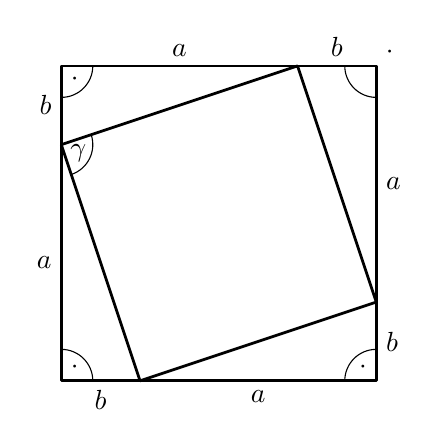
\begin{tikzpicture}
    \tkzSetUpPoint[shape=circle,size=10,color=black,fill=black]
    \tkzSetUpLine[line width=1]
    \tkzDefPoints{0/0/A, 4/0/B, 4/4/C, 0/4/D, 1/0/W, 4/1/X, 3/4/Y, 0/3/Z}
    \tkzDrawPolygon(A,B,C,D)
    \tkzDrawPolygon(W,X,Y,Z)
    \tkzLabelSegment[below](A,W){$b$}
    \tkzLabelSegment[below](W,B){$a$}
    \tkzLabelSegment[right](B,X){$b$}
    \tkzLabelSegment[right](X,C){$a$}
    \tkzLabelSegment[above](C,Y){$b$}
    \tkzLabelSegment[above](Y,D){$a$}
    \tkzLabelSegment[left](D,Z){$b$}
    \tkzLabelSegment[left](Z,A){$a$}
    \tkzLabelAngle[pos=-0.24](D,C,B){$\cdot$}
    \tkzMarkAngle[arc=l,size=0.4cm](D,C,B)
    \tkzLabelAngle[pos=0.24](C,B,A){$\cdot$}
    \tkzMarkAngle[arc=l,size=0.4cm](C,B,A)
    \tkzLabelAngle[pos=0.24](B,A,D){$\cdot$}
    \tkzMarkAngle[arc=l,size=0.4cm](B,A,D)
    \tkzLabelAngle[pos=0.24](A,D,C){$\cdot$}
    \tkzMarkAngle[arc=l,size=0.4cm](A,D,C)
    \tkzLabelAngle[pos=0.24](W,Z,Y){$\gamma$}
    \tkzMarkAngle[arc=l,size=0.4cm](W,Z,Y)
\end{tikzpicture}
\end{document}
